\documentclass[11pt,a4paper]{article}
\usepackage{amsmath,amsthm,amsfonts,amssymb,amscd}
\usepackage{enumerate} 
\usepackage{physics}
\usepackage{enumerate}
\usepackage{fancyhdr}
 \usepackage{hyperref}
\hypersetup{colorlinks,
    linkcolor=blue,
    citecolor=blue,      
    urlcolor=blue,
}
\usepackage{graphicx}


\oddsidemargin0.1cm 
\evensidemargin0.8cm
\textheight22.7cm 
\textwidth15cm \topmargin-0.5cm

\newtheorem{theorem}{Theorem}[section]
\newtheorem{lemma}[theorem]{Lemma}

\usepackage{listings}
\usepackage{xcolor}

\definecolor{codegreen}{rgb}{0,0.6,0}
\definecolor{codegray}{rgb}{0.5,0.5,0.5}
\definecolor{codepurple}{rgb}{0.58,0,0.82}
\definecolor{backcolour}{rgb}{0.95,0.95,0.92}

\lstdefinestyle{mystyle}{
    backgroundcolor=\color{backcolour},   
    commentstyle=\color{codegreen},
    keywordstyle=\color{magenta},
    numberstyle=\tiny\color{codegray},
    stringstyle=\color{codepurple},
    basicstyle=\ttfamily\footnotesize,
    breakatwhitespace=false,         
    breaklines=true,                 
    captionpos=b,                    
    keepspaces=true,                 
    numbers=left,                    
    numbersep=5pt,                  
    showspaces=false,                
    showstringspaces=false,
    showtabs=false,                  
    tabsize=2
}

\lstset{style=mystyle}

\newcommand{\silvia}[1]{{ {\color{blue}{(silvia)~#1}}}}
\newcommand{\grace}[1]{{ {\color{purple}{(grace)~#1}}}}

\pagestyle{fancy}
\fancyhf{}
\lhead{\textsc{Open DP Privacy Proofs: Measurements (Impute)}}
\renewcommand{\headrulewidth}{0pt}
\begin{document}

\vspace{0.2cm}
\emph{Written by Grace Tian}
\vspace{0.2cm}

% \section{Cast}

\section{Impute Uniform Float(TODO)}
 
\subsection{Code in Rust}

Rust code here \url{https://github.com/opendp/opendp/blob/21-impute/rust/opendp/src/trans/impute.rs}

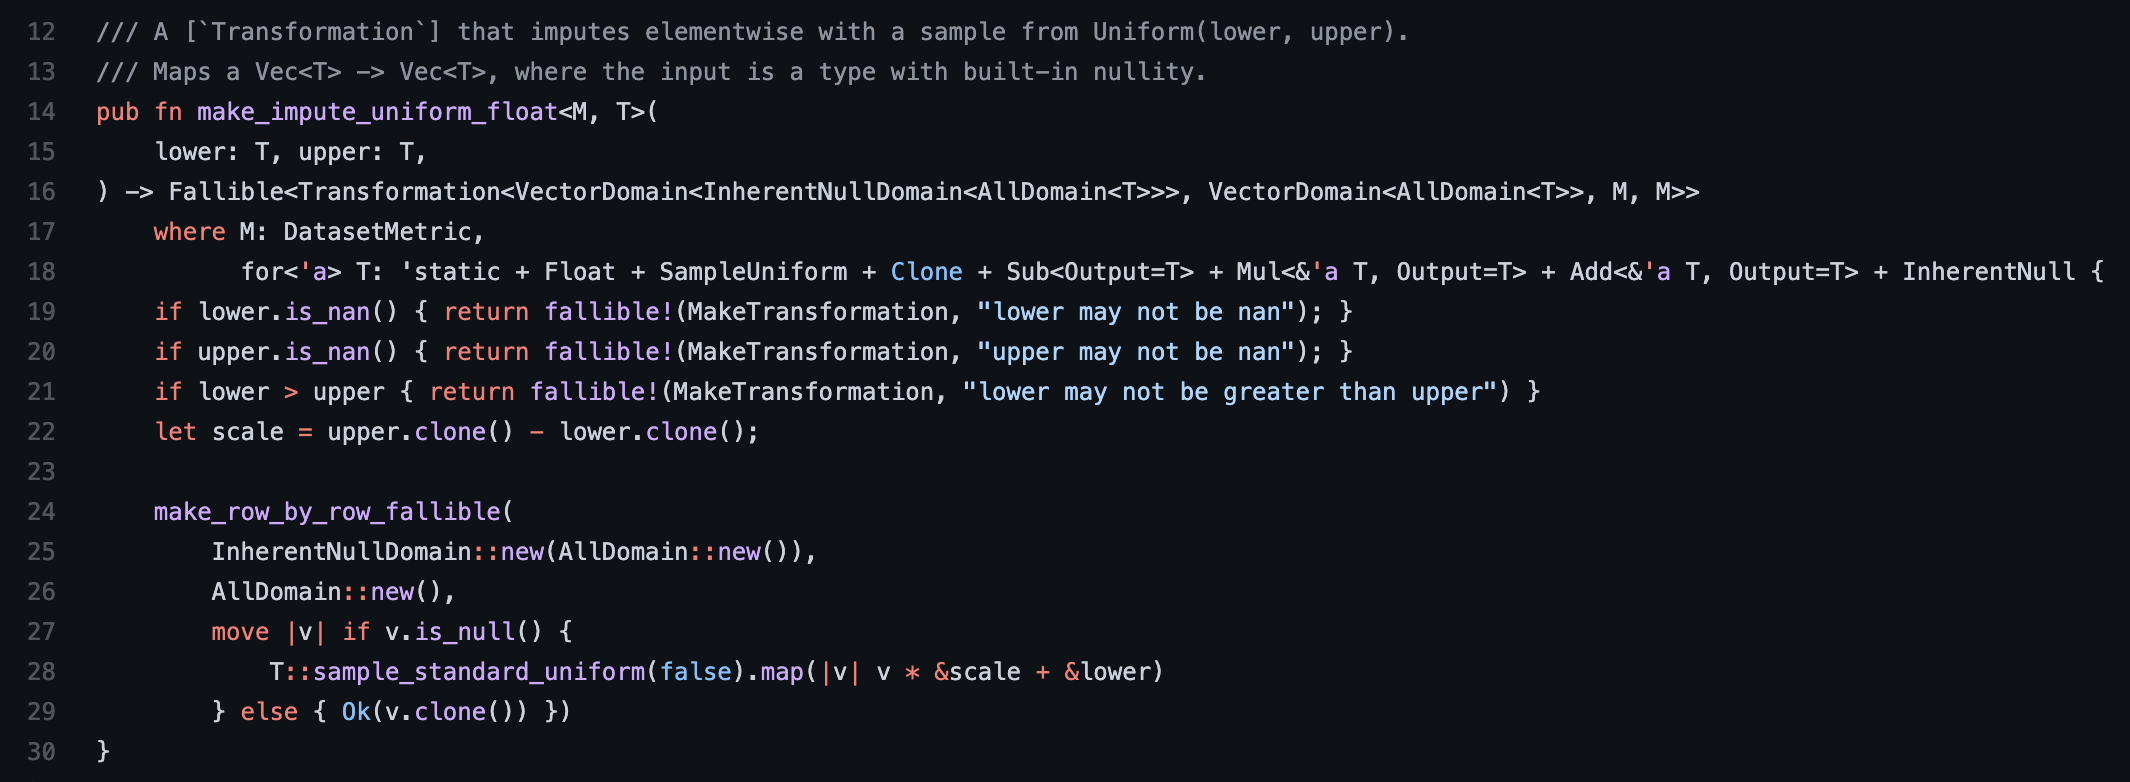
\includegraphics[width=\textwidth]{make_impute_unif_float.png}


\subsection{Pseudo Code in Python}

\textbf{Preconditions}
To ensure the correctness of the output, we require the following preconditions:

\begin{itemize}
    \item \textbf{User-specified types:}
    \begin{itemize}
        \item Variables \texttt{lower} and \texttt{upper} must be of type \texttt{T}
        \item Type \texttt{T} must have traits \texttt{static} \texttt{float}, \texttt{SampleUniform}, \texttt{Clone}, \texttt{Sub(Output=T)}, \texttt{Mul}, \texttt{Add}, and \texttt{InherentNull}.
    \end{itemize}
\end{itemize}

\noindent \textbf{Postconditions}
\begin{itemize}
    \item A \texttt{Transformation} is returned (i.e., if a \texttt{Transformation} cannot be returned successfully, then an error should be returned).
\end{itemize}


\begin{lstlisting}[language=Python]
def make_impute_uniform_float(lower : T, upper : T):
    input_domain = VectorDomain(InherentNullDomain(AllDomain(T)));
    output_domain = VectorDomain(AllDomain(T))
    input_metric = SymmetricDistance()
    output_metric = SymmetricDistance()

    assert .... (TODO);
    
    
    def function(data): 
        return Uniform(lower, upper) if data is null else return data;

    let stability_relation = (d_in <= d_out);
    
    return Transformation(input_domain, output_domain, function, input_metric, output_metric, stability_relation)

\end{lstlisting}






\subsubsection{Conditions as specified in Pseudocode (Delete?)}
\begin{itemize}
    \item Input Domain: all vector domain of type \texttt{T} and null values
    \item Output Domain: all vector domain of type \texttt{bool}
    \item Function: return vector where null values are replaced with Uniform(lower, upper) sampling
    \item Input Metric: Symmetric Distance 
    \item Output Metric: same as Input Metric
    \item Stability Relation: function that takes in 32 bit integers $d_{in}$ and $d_{out}$ and returns whether $d_{in} \leq d_{out}.$
\end{itemize}

\subsection{Proof}
\begin{theorem}
For every setting of the input parameters \texttt{(lower, upper)} to \texttt{make\_impute\_uniform\_float} such that the given preconditions hold, the transformation returned by \texttt{make\_impute\_uniform\_float} has the following properties:
\begin{enumerate}
    \item \textup{(Appropriate output domain).} If vector \texttt{v} in input domain, then \texttt{function(v)} is in output domain.
    \grace{Do I need to say otherwise the program will raise an \texttt{Exception}?}
    
    \item \textup{(Domain-metric compatibility).} The domain \texttt{input\_domain} matches one of the possible domains listed in the definition of \texttt{input\_metric}, and likewise \texttt{output\_domain} matches one of the possible domains listed in the definition of \texttt{output\_metric}.
    \item \textup{(Stability Guarantee).} If two vector inputs $v, w$ are ``$d_{in}$ - close" and if \texttt{Relation($d_{in}$, $d_{out}$) = True} then the corresponding outputs $function(v), function(w)$ are ``$d_{out}$ - close". 
\end{enumerate}
\end{theorem}

\begin{proof}
\begin{enumerate}
    \item \textbf{(Appropriate output domain).} The output correctness follows from the type signature of the function in the rust code. 
    \item \textbf{(Domain-metric compatibility).}
    \item \textbf{(Stability guarantee).}
    
    We know that vectors $v, w$ are $d_{in}$-close, and that $d_{in} \leq d_{out}$ because \texttt{Relation}($d_{in}$, $d_{out}$) \texttt{= True}. By the histogram notation, this means that $$d_{Sym}(v, w) = \norm{h_v - h_w}_1 = \sum_{z} \abs{h_v(z) - h_w(z)} \leq d_{in}.$$ Recall that the \texttt{make\_impute\_uniform\_float} transformation only changes the null values in the vectors $v$ and $w$. Therefore it suffices to consider only the subset of null elements in $Multiset(v)$ and $Multiset(w)$, which we denote respectively as $v^*$ and $w^*$. 
    
    From the histogram notation, we have $h_v(\texttt{null})$ and $h_w(\texttt{null})$ nulls respectively in vectors $v$ and $w$. By the stability for randomness corollary, we can fix the random seed $r$, and say it produces the sequence $(r_1, r_2, r_3, \ldots)$ of randomly generated uniforms from \texttt{Unif(lower, upper)} in this specific order. In other words, the $i$th \texttt{null} in $v$ or $w$ corresponds to $r_i$ in function(v) or function(w). Therefore the symmetric distance of $\textttt{function}(v^*)$ and  $\textttt{function}(w^*)$ is bounded:
    
    
    $$\sum_{r_i \in r} \abs{h_{\texttt{function}(v^*)}(r_i) - h_{\texttt{function}(w^*)}(r_i)} \leq \abs{h_{v}(\texttt{null}) - h_{w}(\texttt{null})}$$
    
    The remaining non-null values in $v$ and $z$ stay the same after the transformation, so the transformations are $d_{out}$-close: $$d_{sym}(\texttt{function}(v), \texttt{function}(w)) = \sum_z \abs{h_{\texttt{function}(v)}(z) - h_{\texttt{function}(w)}(z)}$$
    $$\leq \sum_z \abs{h_v(z) - h_w(z)} \leq d_{in} \leq d_{out}$$ 
    
    


    
\end{enumerate}
\end{proof}

\newpage
\section{Impute Constant (TODO)}
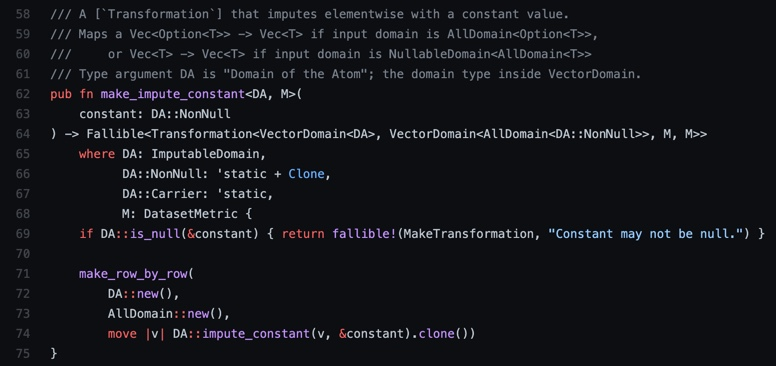
\includegraphics[width=\textwidth]{make_impute_constant.jpg}



\subsection{Pseudo code}



Impute from page 4 in Smart Noise framework: \url{https://github.com/opendp/smartnoise-core/blob/develop/whitepapers/data_processing/data_processing.pdf}




\begin{lstlisting}[language=Python]
def make_impute_constant(constant, input_metric, output_metric):
    let input_domain = VectorDomain<AllDomain<Option<T>>;
    let output_domain = VectorDomain<AllDomain<T>;
    let function(data): return constant;
        
    let stability_relation = (d_out >= d_in);
    
    return Transformation(input_domain, output_domain, function(data?), input_metric, output_metric, stability_relation)

\end{lstlisting}

\section{Proof}
\begin{theorem}
For every setting of the input parameters to \texttt{make\_impute\_constant}, the transformation returned by \texttt{make\_impute\_constant} has the following properties
\begin{enumerate}
    \item \textup{(Appropriate output domain).} If vector \texttt{v} of type \texttt{T} is in the input domain, then \texttt{function(v)} is in the output domain, otherwise the program will raise an \texttt{Exception}. 
    \item \textup{(Stability Guarantee).} If two vector inputs $v, w$ are "$d_{in}$ - close" and if \texttt{Relation($d_{in}$, $d_{out}$) = True} then the corresponding outputs $function(v), function(w)$ are "$d_{out}$ - close". 
\end{enumerate}
\end{theorem}

\begin{proof}
\begin{enumerate}
    \item 
    \item % Stability guarantee

    
    We know that $d_{in} \leq d_{out}$ because \texttt{Relation}($d_{in}$, $d_{out}$) $\texttt{ = True}$. Since the vectors $v, w$ are $d_{in}$-close, then $d_{Sym}(v, w) \leq d_{in}$.
    
    The function transformation just replaces the $\texttt{null}$ element in vectors $v$ and $w$ with \texttt{constant}. Since the null element is also counted toward the symmetric distance of the transformation, the symmetric distance of $\texttt{function}(v)$ and $\texttt{function}(w)$ stays the same. Therefore the transformation is $d_{out}$ close: $d_{sym}(\texttt{function}(v), \texttt{function}(w)) = d_{sym}(v, w) \leq d_{in} \leq d_{out}$
\end{enumerate}

\end{proof}
\end{document}
